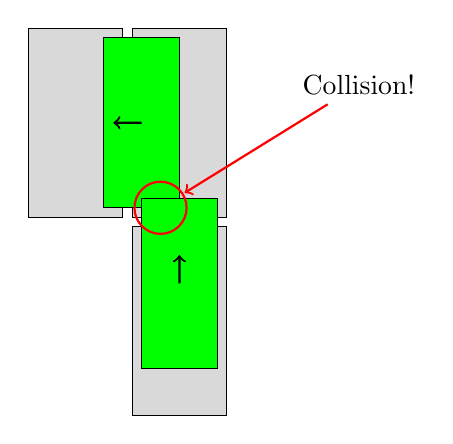
\begin{tikzpicture}[scale=1.2]

\coordinate (A) at (0,2.1);
\coordinate (B) at (1.1,2.1);
\coordinate (C) at (1.1,0);


\foreach \v in {A,B,C}
{
    \draw[fill=gray!30] (\v) + (-0.5,-1) rectangle ++(0.5, 1);
}

\coordinate (D) at (0.7, 2.1);
\coordinate (E) at (1.1, 0.4);

\foreach \v in {D,E}
{
    \draw[fill=green] (\v) + (-0.4,-0.9) rectangle ++(0.4, 0.9);
}

\draw[thick,black,->] (D) -- (0.4,2.1);
\draw[thick,black,->] (E) -- (1.1,0.7);

\node (T) at (3,2.5) {Collision!};
\node[thick, draw, circle, red, scale=2.0] (col) at (0.9,1.2) {};
\draw[thick,red,->] (T) -- (col);

\end{tikzpicture}
